\documentclass{article} % say
\usepackage{tikz}
\begin{document}
La grande ville de Karwa-sur-mer souhaite moderniser les buildings présent sur la digue. En effet la ville veut poser des panneaux solaires sur ceux-ci et afin de profiter un maximum de la production électrique de ceux-ci, elle décide de recouvrir bien évidemment les toits des batiments et les facades de côtés. L'idée étant de profiter du soleil du matin au soir.


Pour cela vous êtes engagé afin de déterminer combien de mètres de panneaux la ville aura besoin pour équiper ses batiments. La ville vous donne pour cela un plan en vue de face de la digue vous spécifiant la taille des bâtiments comme ceci : \\

Pour chaque emplacement de 1 mètre de large, le plan vous donne la hauteur du batiments à cet emplacement comme illustré par la figure ci-dessous.

\begin{figure}[h]
\centering
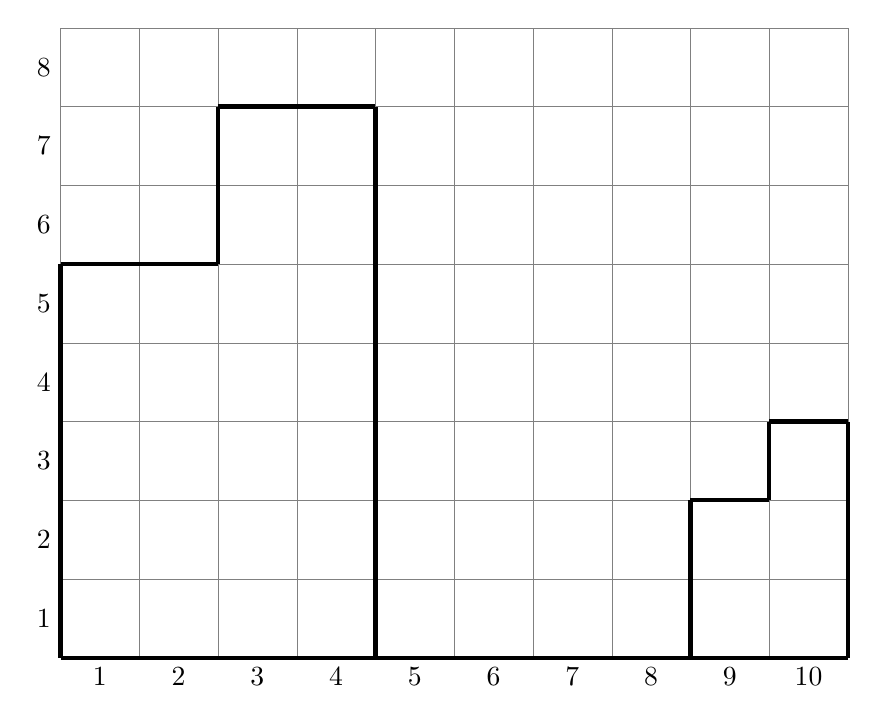
\begin{tikzpicture}
\draw[step=1.0, gray, ultra thin] (0,0) grid (10, 8);
\draw [ultra thick] (0,0) -- (10, 0);

  \draw[ultra thick] (0,0) -- (0, 5);
  \draw[ultra thick] (0, 5) -- (2, 5);
  \draw[ultra thick](2,5) -- (2, 7);
  \draw[ultra thick](2, 7) -- (4, 7);
  \draw[ultra thick](4,7) -- (4, 0);
  \draw[ultra thick](4, 0) -- (8, 0);
  \draw[ultra thick](8,0) -- (8, 2);
  \draw[ultra thick](8, 2) -- (9, 2);
  \draw[ultra thick](9, 2) -- (9, 3);
  \draw[ultra thick] (9, 3) -- (10, 3);
  \draw[ultra thick] (10, 3) -- (10, 0);
    \foreach \x in {1, ..., 10} {%
      % Bottom
      \node[anchor=north] at (\x-0.5,0) {\x};
    }
    
    \foreach \y in {1, ..., 8} {%
      % Left
      \node[anchor=east] at (0,\y-0.5) {\y};
    }
\end{tikzpicture}
\newline
\textit{Illustration de l'exemple 1}
\end{figure}


\section*{Inputs}
Vous recevrez 2 lignes :
La première contient un entier $n$ tel que $1 \leq n \leq 10 000$, la longueur en metre de la digue.
La seconde ligne représente la ligne d'horizon composé de $n$ entiers $h_{i}$ séparé d'un espace représentant la hauteur du batiment en position $i$. Notez que $0 \leq h_{i} \leq 100$

\section*{Output}
Vous devez afficher un seul entier représentant le nombre de mètre de panneaux nécessaire afin de recouvrir la totalité des côtés et dessus des batiments.
\end{document}tikz}

%%% Local Variables:
%%% mode: latex
%%% TeX-master: t
%%% End:
